


\subsection{ISM Dust Grains}

The disk's mass is 99\% made up of gas, and the other 1\% is dust \citep{Birnstiel2016}. The dust that is now in the disk is originally from the interstellar medium (ISM), is the raw material that will make up terrestrial planets, and the cores of giant planets \citep{Williams}. Dust in the ISM is typically sub-micron in size \citep{Williams} and made up of silicate, carbonaceous and icy particles \citep{Testi}. 



\subsection{Grain Growth}
Although dust only accounts for 1\% of the disks initial mass, its evolution plays a vital role in the evolution of the disk and the formation of planets \citep{Williams}. The first step in planet formation is called grain growth, sometimes called dust coagulation \citep{Kataoka_2015}. Grain growth refers to the process where transport mechanisms in the disk lead to many grain-grain collisions, where the grains stick together and form a larger particle \citep{Testi}. During this phase, the grains begin as micron-sized particles and grow to centimetres in size and larger, and become planetesimals  \citep{Testi}. This process is highlighted in the bottom right of Figure \ref{fig: dust-grain-growth-schematic}. 

\question{Should I go into more detail about how this happens? turbulent mixing, settling, drift, etc \citep{Testi}} \note{If so, there is a much better image in \cite{Testi} that I can swap out for Figure \ref{fig: dust-grain-growth-schematic}}. 

\begin{figure*}[h]
  \centering
  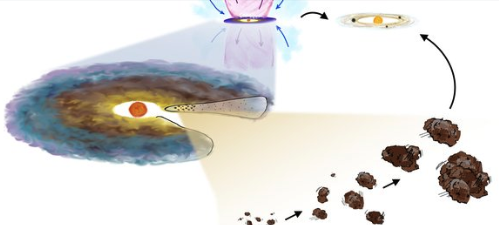
\includegraphics[width=0.8\textwidth]{../IMAGES/SLIDESHOW_SCREENSHOT/dust_grain_growth_schematic.png}
  \caption{Schematic of dust grain growth, the first stage of planet formation. \add{reference} \note{If keeping this image, I will get a higher resolution version, and ask for permission.}}
  \label{fig: dust-grain-growth-schematic}
\end{figure*}

%%%%%%%%%%%%%%%%%%%%%%%%%%%%%%%%%%%%%%%%%%%%%%%%%%%
%%%%%%%%%%%%%%%%%%%%%%%%%%%%%%%%%%%%%%%%%%%%%%%%%%%
\subsection{Effects of Grain Size on Observed Emission}
\label{sec: intro_dust_grainsize}

Dust grains dominate the opacity in the disk, controlling how radiation is absorbed, scattered and emitted \citep{Williams}. The opacity depends on several properties of the dust, including its shape, composition and size \citep{Kataoka_2015}. 

% Different grain sizes absorb radiation differently
At millimetre wavelengths, the continuum emission from disks is dominated by thermal emission from the dust, which is controlled by the opacity of the dust \citep{Testi}. The efficiency with which the dust grains absorb and emit radiation depends on their size relative to the observing wavelength  \citep{Testi}. 

% Different grain sizes scatter radiation differently 
Grain size also affects the scattering properties of dust. Smaller grain sizes at millimetre wavelengths are less efficient at scattering light \citep{Kataoka_2015}. However, larger grain sizes that are close to the observing wavelength are much more efficient at scattering light \citep{Kataoka_2015}.

Because the absorption and scattering properties of dust grains depend on their size relative to the observing wavelength, observations at millimetre wavelengths can be used to study dust grain growth in disks \citep{Testi}. 





%-------------------------------------------





% \quoted{Consequently, dust determines the observational appearance of the disk: on one hand through its thermal continuu, emission and on the other hand by determining the temperature and density structyure and therefore the excitation conditions for gas lines }\citep{Birnstiel2016}. 


% \qupted{Understanding the evolution of solids is a key element in the pizzle of planet formation} \citep{Birnstiel2016}. 


% Determining the grain sizes from observations of disks is important to understand this first stage of planet formation \citep{Kataoka_2015}.



% \quoted{If the grains are large sufficiently large, they have a large scattering opacity, and there is a significant amount of scattered light component in the dust continuum emission \cite{Kataoka_2015}.} 